%% osm-applications.tex
%%


\section{Applications}

\frame[plain]{  \heading{Plan de la Présentation}
\ecmsetupplan
\begin{itemize}
  \item[\small $\Diamond$] Introduction
  \item[\small $\Diamond$] Fonctionnement 
  \item[\small $\Diamond$] {\color{purple}\textbf{Applications}}
  \item[\small $\Diamond$] Technique
  \item[\small $\Diamond$] Communauté
  \item[\small $\Diamond$] Conclusions
\end{itemize}
}



\frame{\centering OpenCycleMap.org\newline\vfil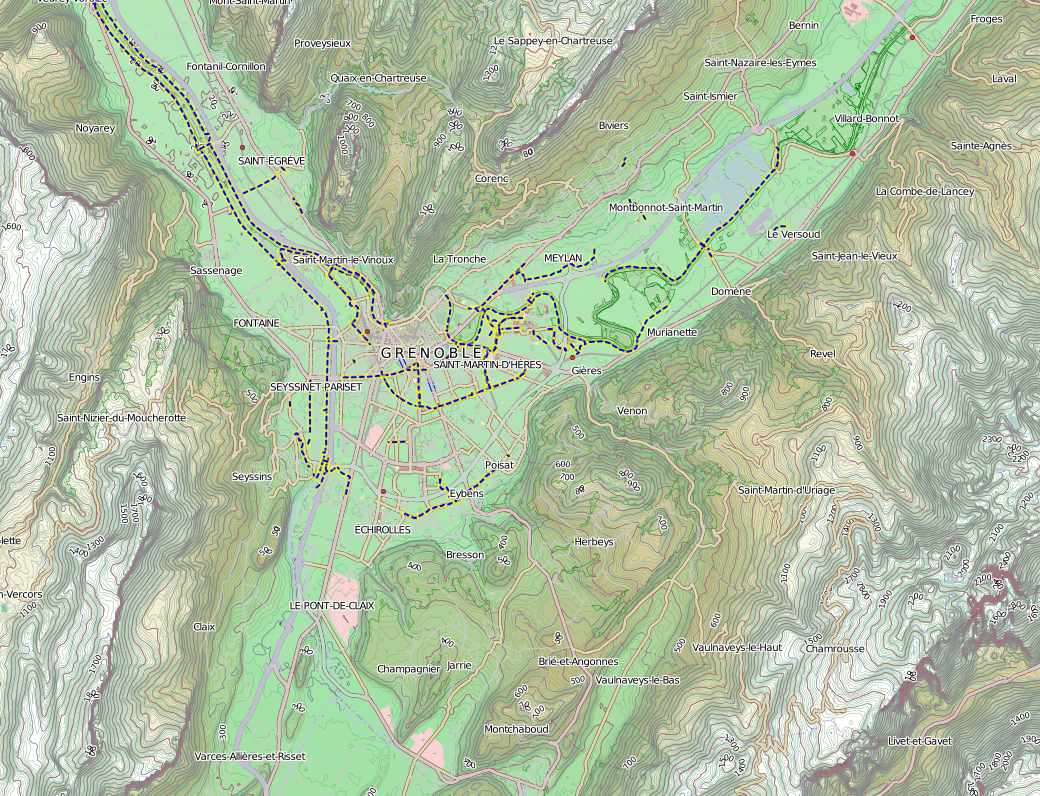
\includegraphics[width=0.95\textwidth]{figures/open-cycle-map}}
\frame{\centering Letuffe.org Hiking\newline\vfil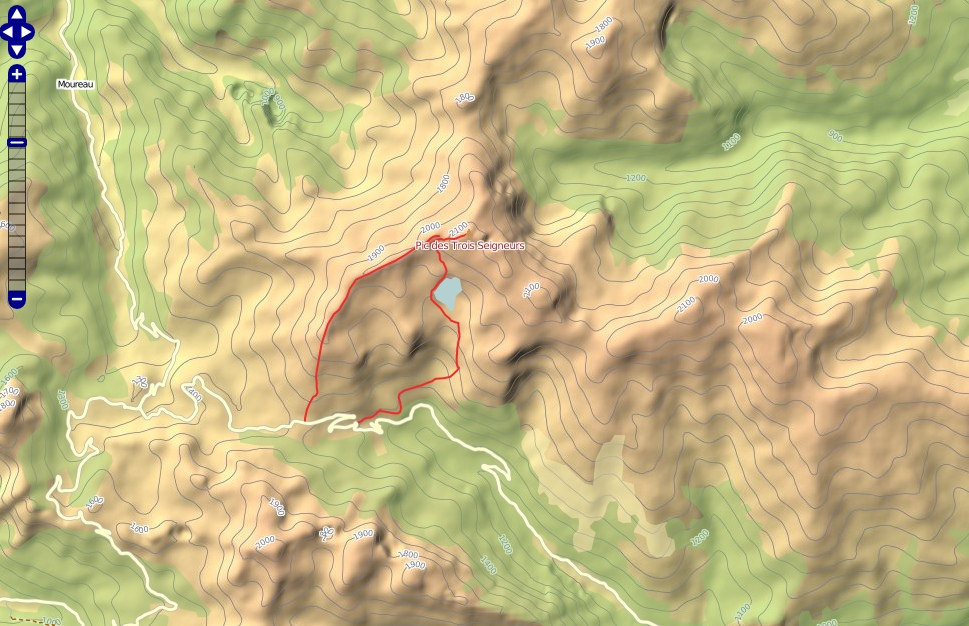
\includegraphics[width=0.95\textwidth]{figures/hiking-letuffe}}
\frame{\centering OpenPisteMap.org\newline\vfil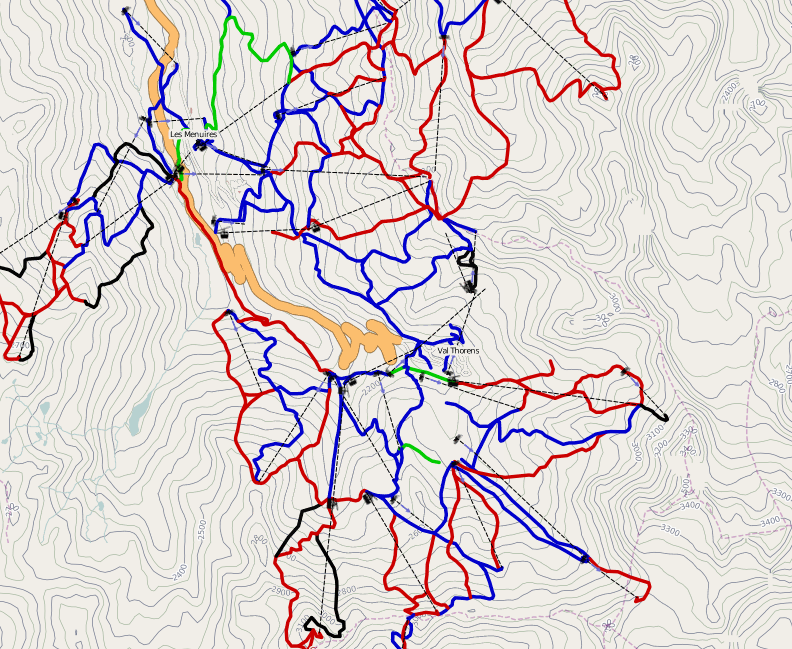
\includegraphics[height=0.94\textheight]{figures/open-piste-map}}
\frame{\centering öpenvkarte.de\newline\vfil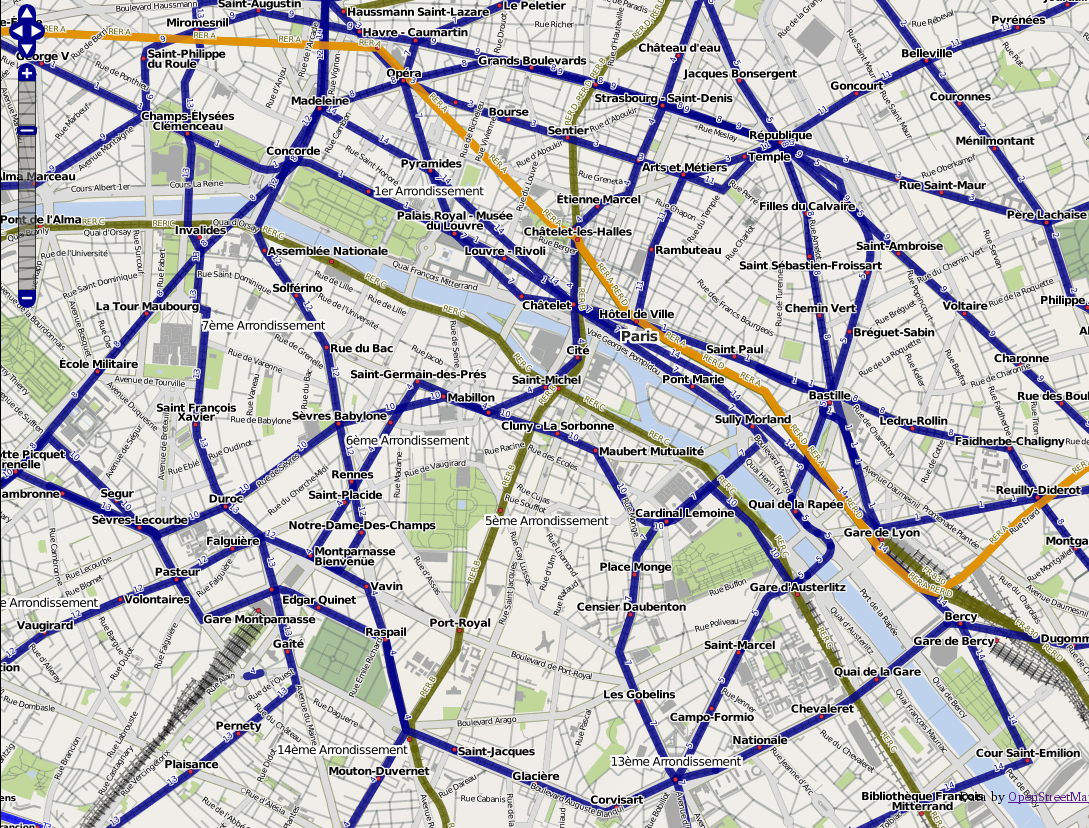
\includegraphics[width=0.98\textwidth]{figures/opnvkarte}}
\frame{\centering OpenSeaMap.org\newline\vfil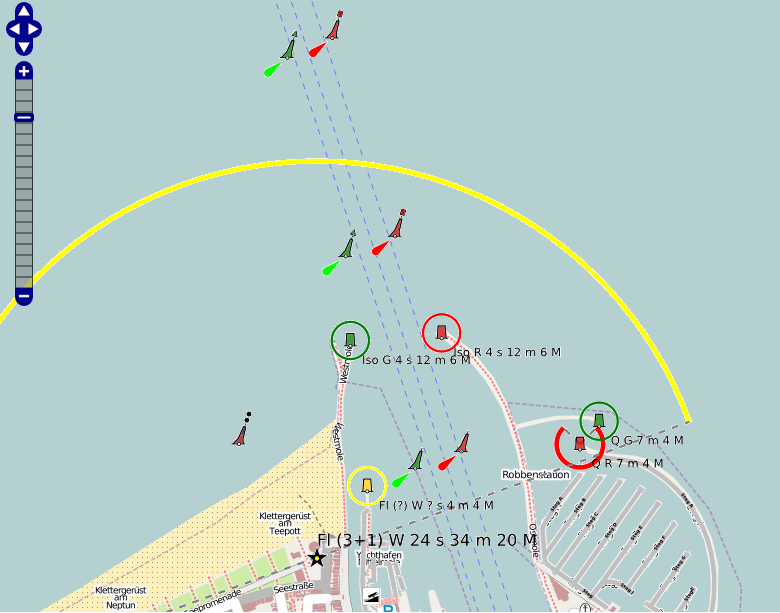
\includegraphics[width=0.98\textwidth]{figures/open-sea-map}}
\frame{\centering osm-wms.de\newline\vfil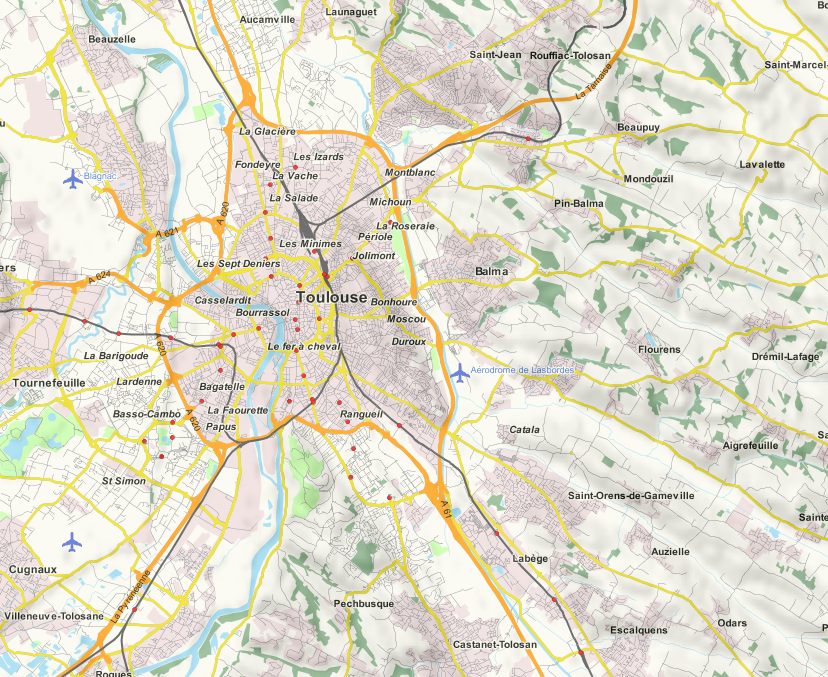
\includegraphics[width=0.98\textwidth]{figures/OSM-WMS}}
\frame{\centering TopOSM.com\newline\vfil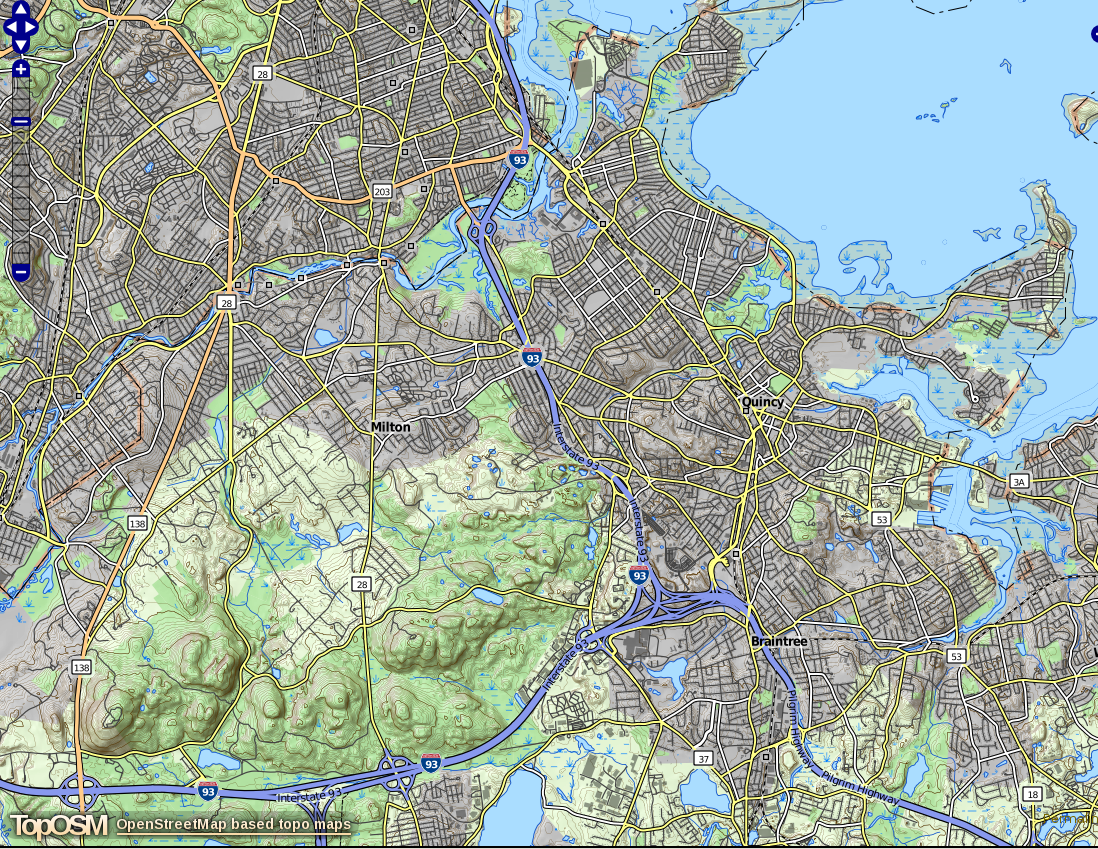
\includegraphics[width=0.99\textwidth]{figures/toposm}}


\frame { \heading{MapOSMatic -- plans de ville} \vfill
  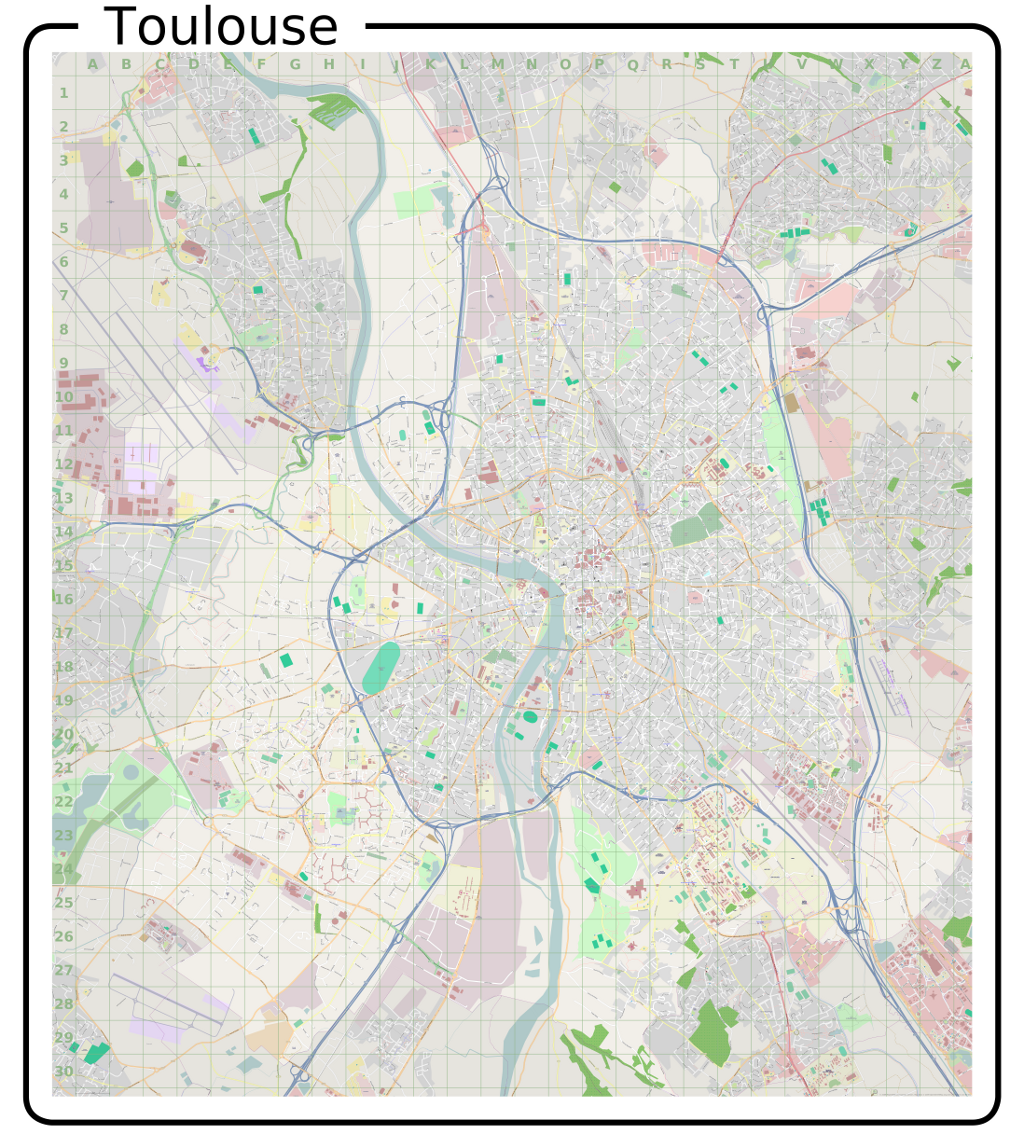
\includegraphics[width=0.47\textwidth]{figures/maposmatic-toulouse} \quad %
  \includegraphics[width=0.47\textwidth]{figures/maposmatic-toulouse-index}
}


\frame{\heading{Carte touristique de Gaza} \vfill
  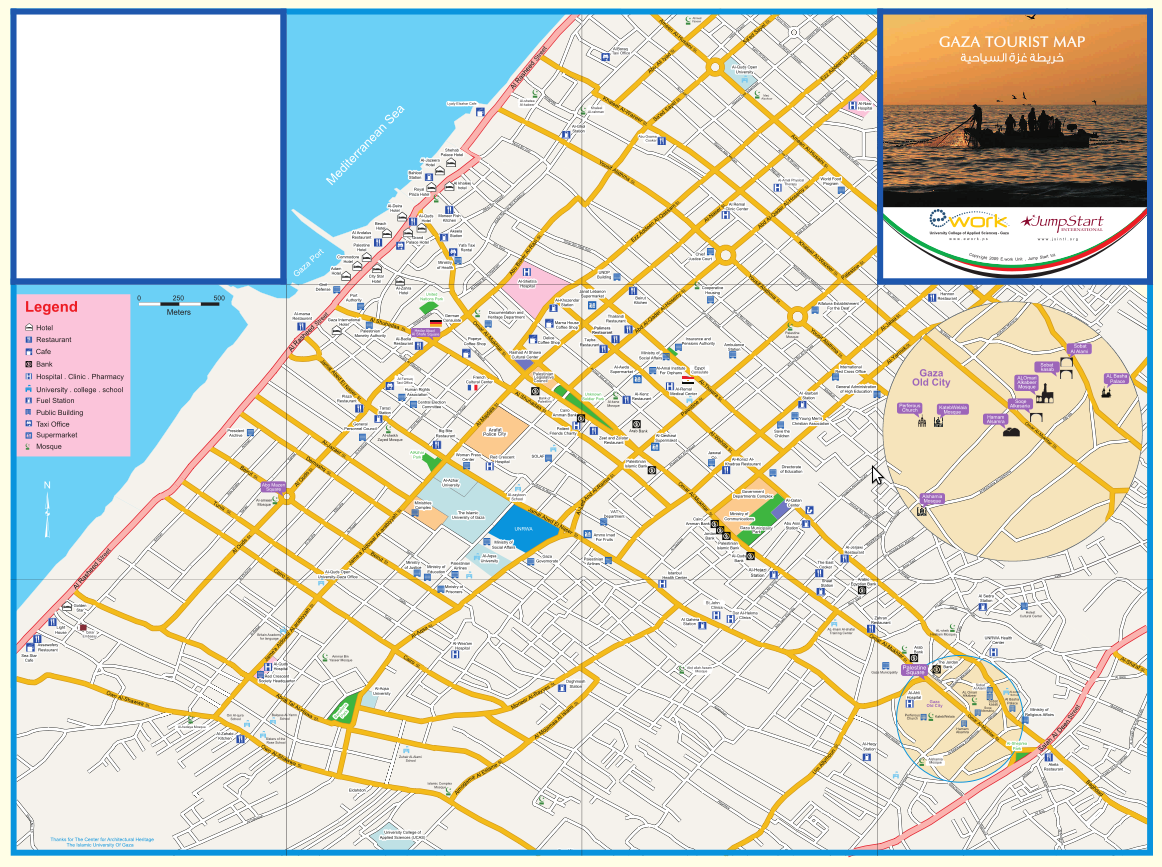
\includegraphics[width=0.9\textwidth]{figures/Gaza_tourist}
}

\frame{\heading{Carte du slum Kibera (Nairobi, Kenya)} \vfill
  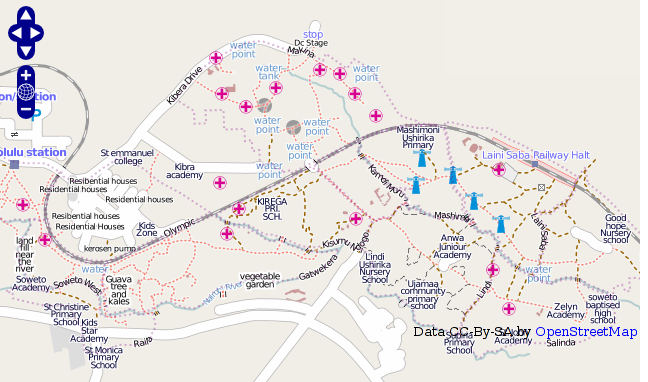
\includegraphics[width=0.9\textwidth]{figures/osm-kibera}
}


\frame{ \heading{Utilisation sur terminal mobile} \vfil
  \begin{tikzpicture}[remember picture,overlay,font={\footnotesize},text
    width=2cm,text centered]
   \node[xshift=1cm,yshift=-4cm] at (current page.north west) {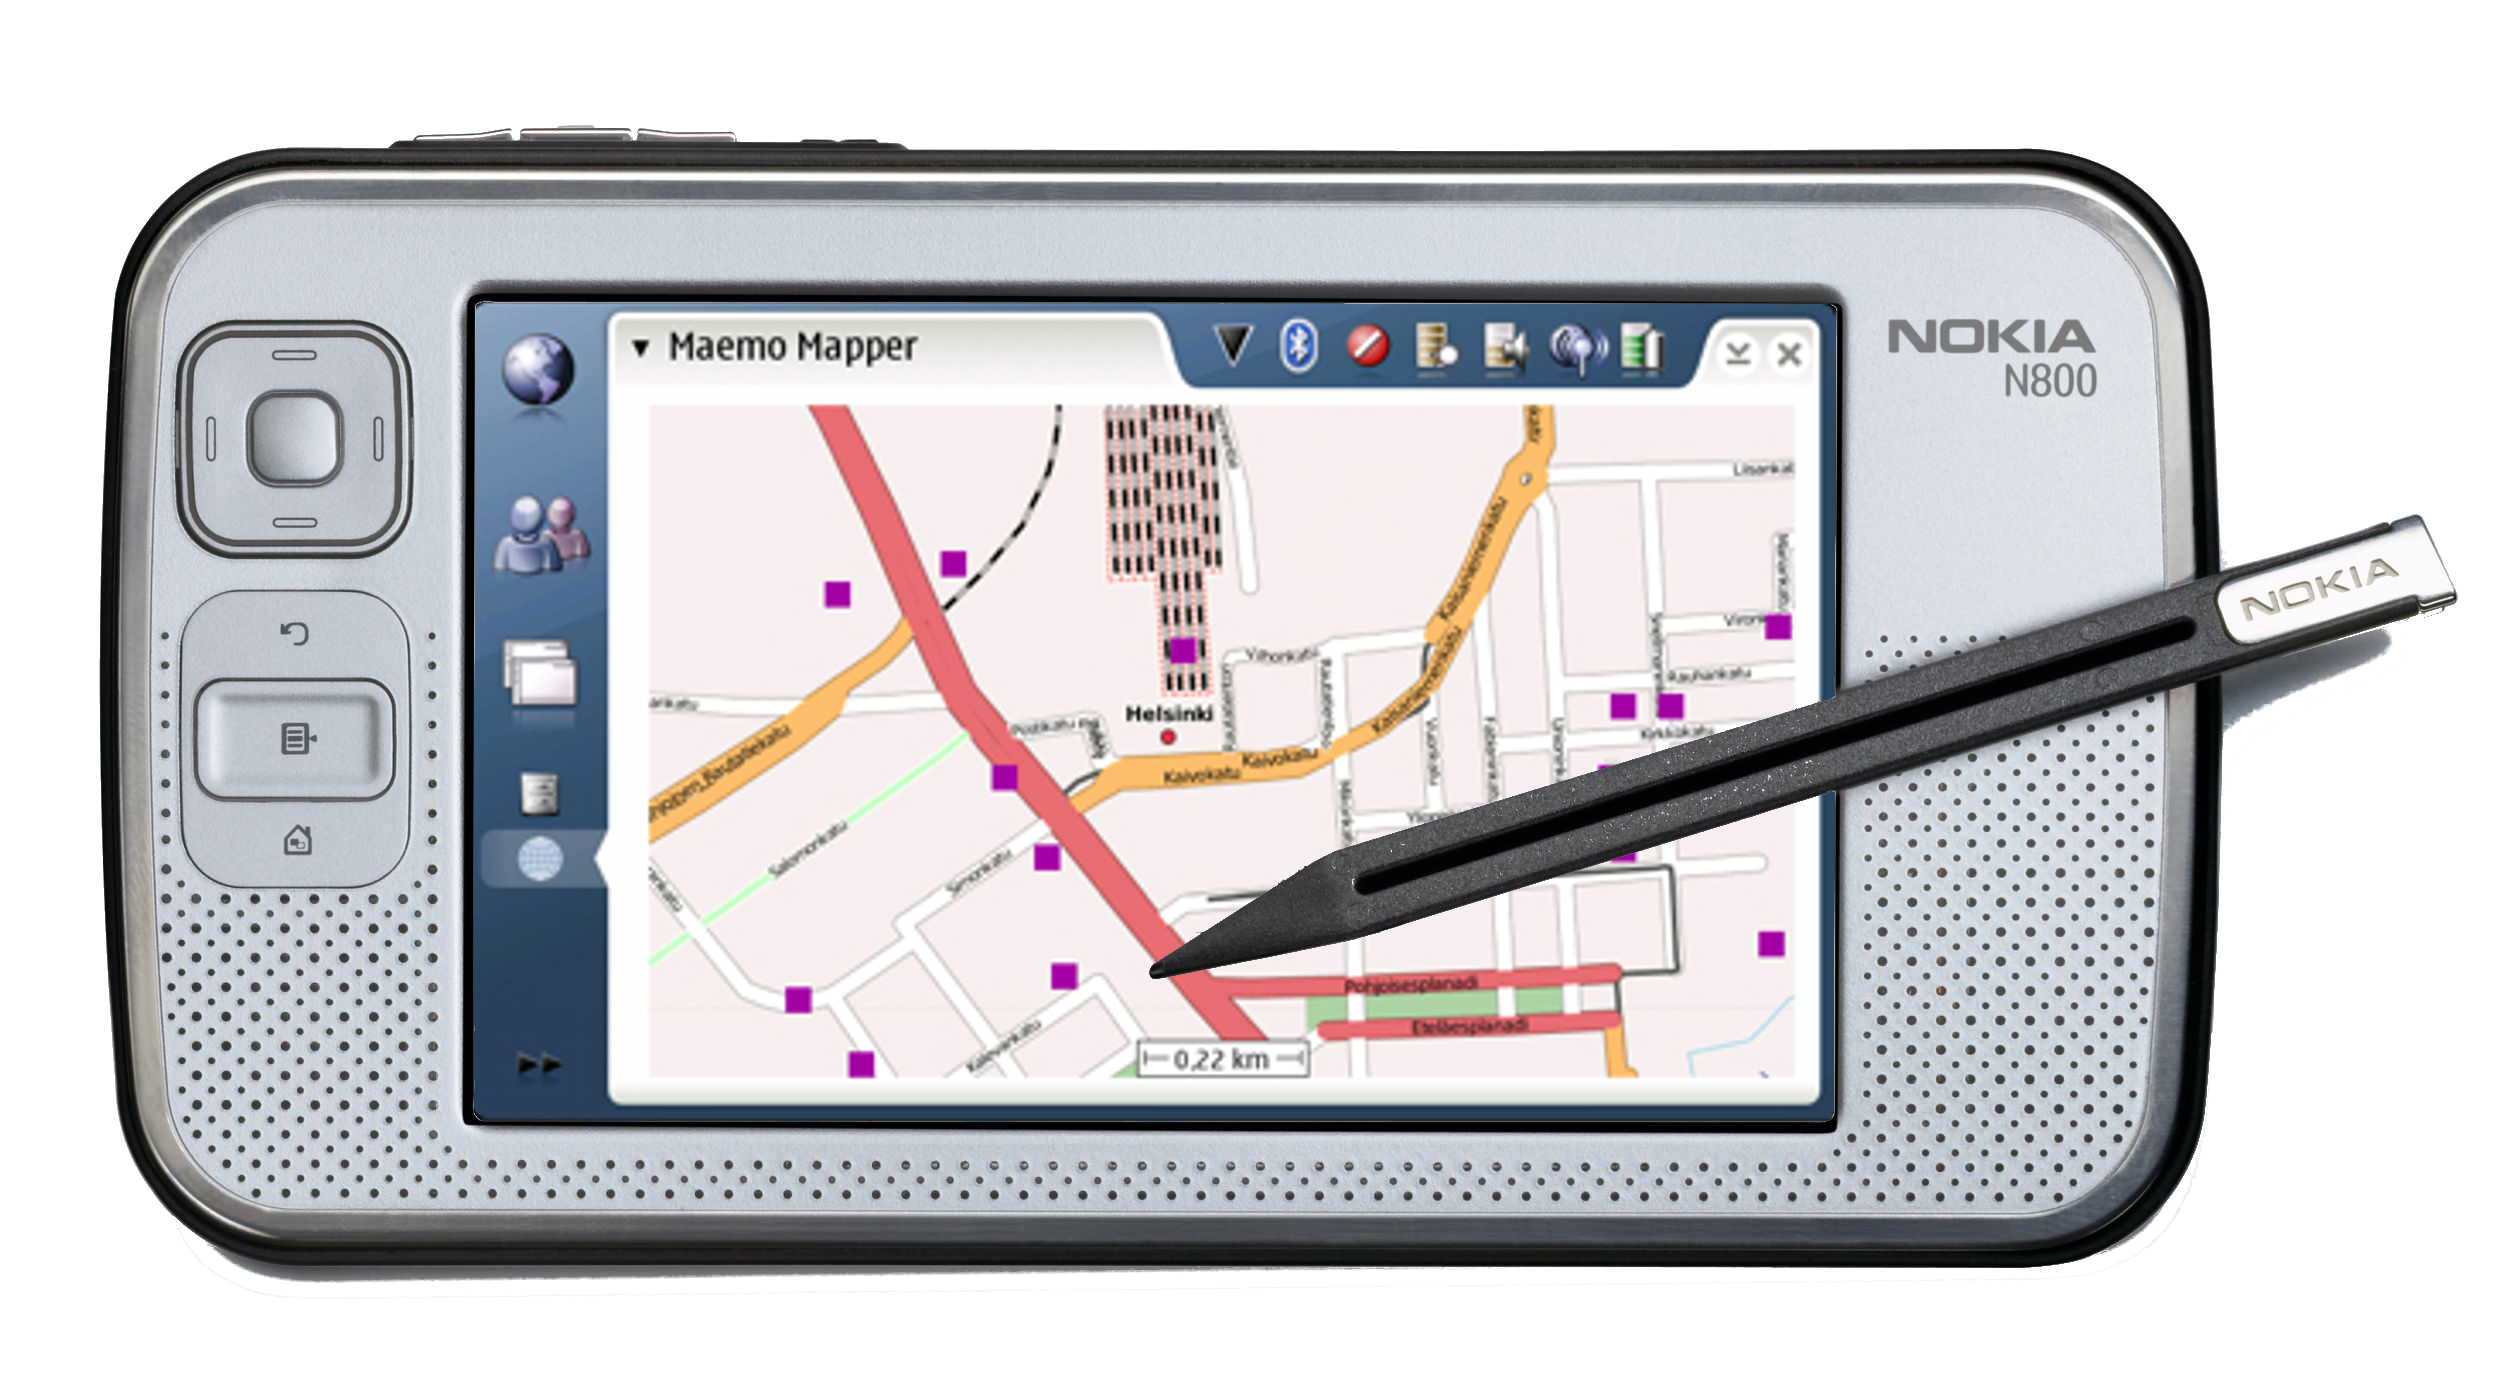
\includegraphics[width=7cm]{figures/osm-N800}};
   \node[xshift=-1cm,yshift=-3cm] at (current page.north east) {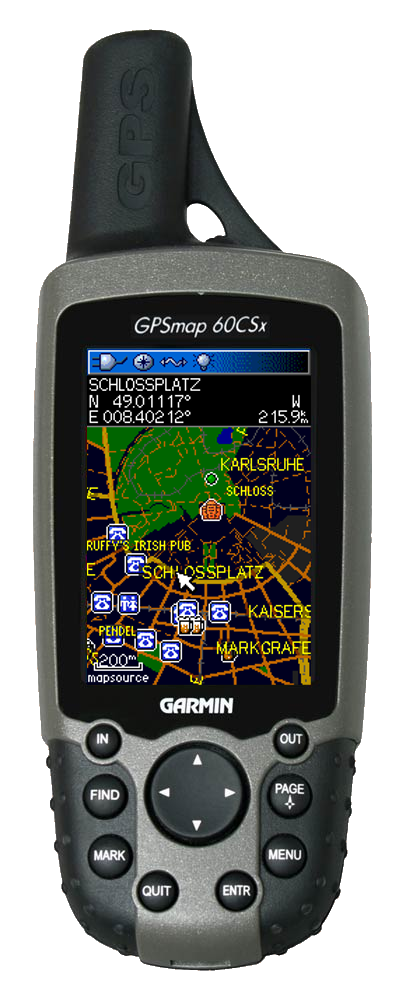
\includegraphics[height=5cm]{figures/OSM-garmin}};
   \node[xshift=-4.7cm,yshift=3.5cm] at (current page.south east) {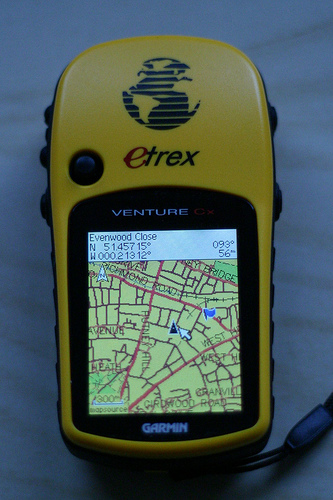
\includegraphics[height=5cm]{figures/OSM-garmin-etrex}};
\end{tikzpicture}
}



\frame{ \heading{Utilisation sous Android} \vfil

 \begin{tikzpicture}[remember picture,overlay,font={\footnotesize},]
   \node[xshift=2cm,yshift=-4cm] at (current page.north west)
        {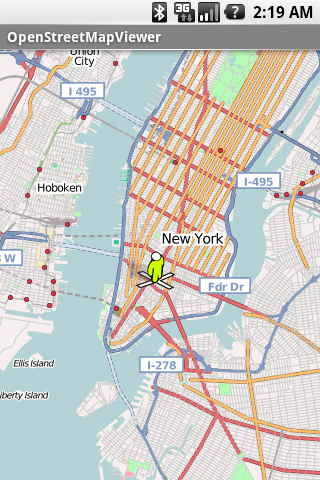
\includegraphics[width=0.3\textwidth]{figures/osm-android-viewer}};
   \node[xshift=-2.5cm,yshift=-3cm] at (current page.north east)
        {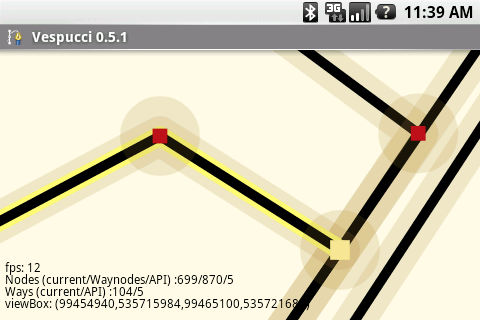
\includegraphics[width=0.4\textwidth]{figures/osm-vespucci}};
   \node[xshift=-6.7cm,yshift=3cm] at (current page.south east)
        {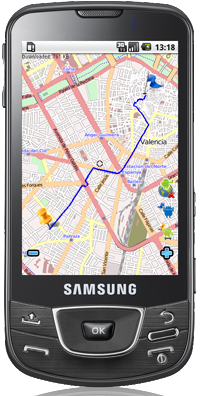
\includegraphics[width=0.25\textwidth]{figures/osm-gvsig} gvSIG};
\end{tikzpicture}
}


%% http://www.foss4g2007.org/presentations/view.php?abstract_id=56


\frame { \heading{Utilisations des données} \vfil

  %% http://www.osm-3d.org/
  
  %% http://wiki.openstreetmap.org/index.php/Fr:Using_OpenStreetMap
  
  %% http://wiki.navit-project.org/images/thumb/f/fa/FBZH-gtk.png/800px-FBZH-gtk.png
  
  \begin{minipage}{0.8\textwidth}
  \begin{itemize}
  \item guidage temps réel (applications: navit, GPSDrive, gosmore, roadnav) 
  \item cartes et applications de routage thématiques
    \begin{itemize}
    \item spécifique vélo ou piéton ou bâteau
    \item carte des châteaux d'une zone viticole
    \item préparation d'un \textit{pub crawl}
    \item une association de commerçants qui produit son plan de la ville
    \end{itemize}
  \item une petite mairie qui voudrait un GIS de sa commune sans
        pouvoir payer tous les ans une licence commerciale
  \item étudiants ou chercheurs voulant travailler sur des données géographiques
  \item utiliser les données dans des simulateurs
    \begin{itemize}
    \item existe pour FlightGear (avec terragear)
    \end{itemize}

  \item insérer votre idée ici: les données sont libres!
  \end{itemize}
  \end{minipage} %
  \begin{minipage}{0.19\textwidth}
    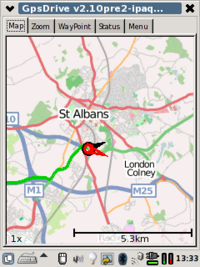
\includegraphics[width=1.5cm]{figures/200px-Gpsdrive_ipaq_screenshot-map-z11}
    \vskip 1cm

    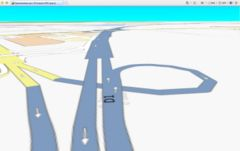
\includegraphics[width=1.5cm]{figures/240px-Now_turn_right2}
    \vskip 1cm
    
    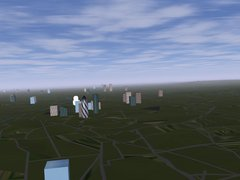
\includegraphics[width=1.5cm]{figures/240px-Osmroads1}
    \vskip 1cm
  \end{minipage}
}



% ** – Un étudiant qui veut tester les algorithmes de plus court chemin
% qu'il vient d'apprendre à l'école sur des données réelles
% – Une association de défense du vélo qui voudrait calculer des
% itinéraires adaptés au vélo ;)
% – Une petite mairie qui voudrait avoir un GIS de sa commune sans
% pouvoir payer tous les ans une licence Navteq ou quelqu'un pour mettre
% à jour les données.  J'ai un exemple concret avec le SDIS-31
% (pompiers) qui se basent sur une vieille carto Navteq et une personne
% qui travaille pratiquement à temps plein pour corriger les erreurs de
% la carte et mettre à jour les modifications. Avec OSM ils auraient
% économisé une partie du boulot.
% - Un militant qui crée son analyse de données OSM (beta.letuffe, osmose,
% mais dans d'autres domaines : p.ex calcul de espaces verts par commune)
% - Un passionné qui crée sa carte animée sur données OSM (Opentransport
% animé : il y avait une carte suisse avec les trains en mouvement, sur
% fond Google, mais je n'ai plus l'adresse)
% - Une association culturelle qui imprime sa carte locale des sites
% médiévaux,
% - Une association de commerçants qui produit son plan de la ville.
% - Un service culturel/syndicat d'initiative/Office du tourisme qui
% propose une carte web des événements à venir sur la commune (
% - Un enseignant qui fournit des fonds de cartes, des contours des
% collectivités à ses élèves (grâce à mapOSthéMatic ou géosmgraphie.org ;-)



%% http://www.geographie.uni-bonn.de/karto/osm-3d/screenshots.en.htm

%% EOF
